\begin{frameExample}{Planeación de la Producción}{}
  % EXAMPLE 2.6-9 (Production Planning Problem) 
Una fábrica elabora un producto cuya unidad consta de 5 unidades de la parte A y 4 unidades de la parte B. Las dos partes A y B requieren diferentes materias primas, de las cuales están disponibles 120 unidades y 240 unidades respectivamente. Estas piezas pueden fabricarse por tres métodos diferentes. Los requisitos de materia prima por producción y el número de unidades para cada parte producida se detallan a continuación. Formule el modelo L.P. para determinar el número de corridas de producción para cada método a fin de maximizar el número total de unidades completas del producto final.

{\centering
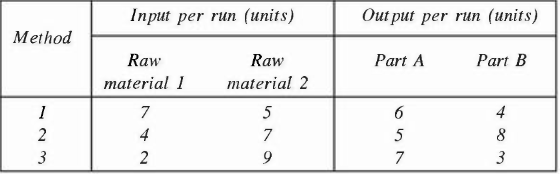
\includegraphics[scale=0.5]{example_production-planning_gupta}
\par}


\end{frameExample}



%%% Local Variables:
%%% mode: latex
%%% TeX-master: "../slides"
%%% End:
